\hypertarget{aquisiuxe7uxe3o-e-tratamento-de-dados}{%
\chapter{Aquisição e Tratamento de Dados}\label{aquisiuxe7uxe3o-e-tratamento-de-dados}}

\section*{Objetivos de Aprendizagem}

Ao final deste capítulo, o leitor será capaz de:

\begin{itemize}
\tightlist
\item
  Descrever a cadeia completa de aquisição, do fenômeno físico ao valor gravado no histórico.
\item
  Escolher o tipo de sinal e a forma de conexão adequados a cada medição.
\item
  Explicar resolução, exatidão e ruído e distinguir um do outro na prática da instalação.
\item
  Justificar as taxas de varredura de cada elo e reconhecer quando um evento se perde entre eles.
\item
  Aplicar tratamento de dados: filtração, validação de faixa, faixa morta e publicação por exceção.
\item
  Projetar o registro da primeira falha de uma parada de planta.
\end{itemize}

\begin{center}\rule{0.5\linewidth}{0.5pt}\end{center}

\hypertarget{a-cadeia-de-aquisiuxe7uxe3o}{%
\section{A cadeia de aquisição}\label{a-cadeia-de-aquisiuxe7uxe3o}}

Nenhum dado industrial nasce pronto. Entre o fenômeno físico e o número que o historiador grava
existe uma cadeia de elos, e cada elo degrada, atrasa ou descarta informação. Conhecer a cadeia é o
que permite diagnosticar por que o valor na tela não corresponde ao que aconteceu no processo.

\begin{center}
\IfFileExists{../figuras/capitulo-15-m1.pdf}{%
  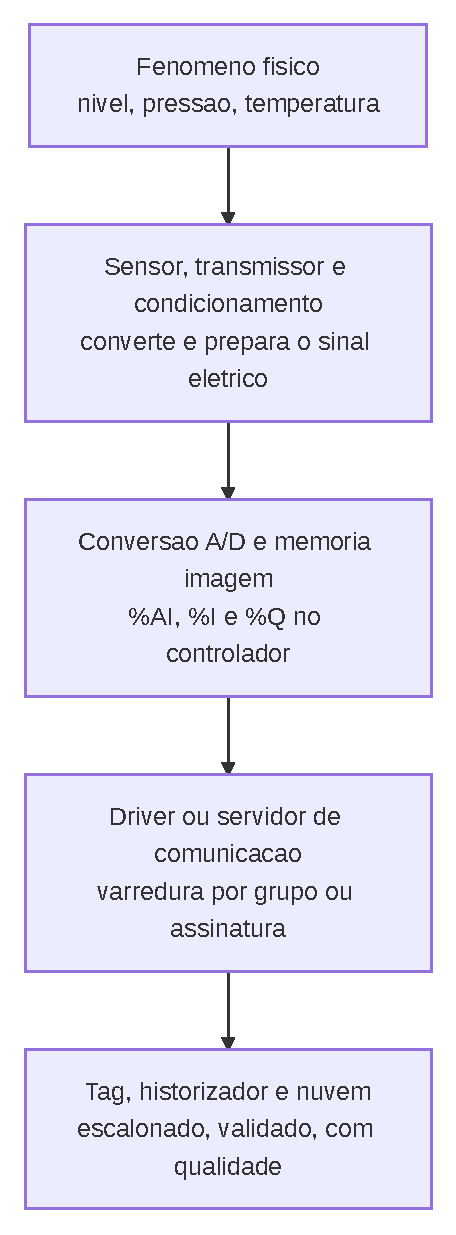
\includegraphics[width=\linewidth,height=0.8\textheight,keepaspectratio]{../figuras/capitulo-15-m1.pdf}%
}{\fbox{\parbox{0.9\linewidth}{\small Diagrama Mermaid ainda não renderizado: capitulo-15-m1. Rode scripts/render-mermaid.sh.}}}
\end{center}

\textbf{Tabela 15.1 -- O que cada elo pode fazer com o dado}

\begin{longtable}[]{@{}
  >{\raggedright\arraybackslash}p{(\columnwidth - 4\tabcolsep) * \real{0.3333}}
  >{\raggedright\arraybackslash}p{(\columnwidth - 4\tabcolsep) * \real{0.3333}}
  >{\raggedright\arraybackslash}p{(\columnwidth - 4\tabcolsep) * \real{0.3333}}@{}}
\toprule\noalign{}
\begin{minipage}[b]{\linewidth}\raggedright
Elo
\end{minipage} & \begin{minipage}[b]{\linewidth}\raggedright
O que ele acrescenta
\end{minipage} & \begin{minipage}[b]{\linewidth}\raggedright
Como ele degrada
\end{minipage} \\
\midrule\noalign{}
\endhead
\bottomrule\noalign{}
\endlastfoot
Sensor e transmissor & Converte a grandeza física em sinal elétrico & Erro de exatidão, deriva, tempo de resposta do próprio sensor \\
Condicionamento & Filtra ruído, isola, protege contra surto & Filtro mal dimensionado atrasa a resposta e suaviza o evento \\
Conversor A/D & Quantifica o sinal em degraus discretos & Perde resolução se a faixa utilizada for muito maior que o sinal \\
Memória imagem & Mantém o valor atual no controle & É sobrescrita a cada varredura: o que não é copiado, desaparece \\
Driver e rede & Transporta em blocos, com taxa configurável & Atraso e perda sob congestionamento; ordem de chegada fora de sequência \\
Tag e historizador & Escalona, valida, filtra e arquiva & Descarta por faixa morta, por validação ou por política de retenção \\
\end{longtable}

\begin{caixanota}

\textbf{Nota:} o elo mais barato de corrigir quase nunca é o transmissor. Antes de trocar um
instrumento, verifique a faixa configurada, o filtro do canal, o endereço no mapa de memória e a
taxa de varredura --- os mesmos quatro itens que explicam a maior parte das reclamações de ``leitura
errada''.

\end{caixanota}

\begin{center}\rule{0.5\linewidth}{0.5pt}\end{center}

\hypertarget{tipos-de-sinal-e-forma-de-conexuxe3o}{%
\section{Tipos de sinal e forma de conexão}\label{tipos-de-sinal-e-forma-de-conexuxe3o}}

A escolha do sinal determina o custo do cabeamento, a imunidade a ruído e o que é possível fazer com
o dado depois. As formas mais usadas:

\textbf{Tabela 15.2 -- Comparativo dos sinais de campo}

\begin{longtable}[]{@{}
  >{\raggedright\arraybackslash}p{(\columnwidth - 8\tabcolsep) * \real{0.2000}}
  >{\raggedright\arraybackslash}p{(\columnwidth - 8\tabcolsep) * \real{0.2000}}
  >{\raggedright\arraybackslash}p{(\columnwidth - 8\tabcolsep) * \real{0.2000}}
  >{\raggedright\arraybackslash}p{(\columnwidth - 8\tabcolsep) * \real{0.2000}}
  >{\raggedright\arraybackslash}p{(\columnwidth - 8\tabcolsep) * \real{0.2000}}@{}}
\toprule\noalign{}
\begin{minipage}[b]{\linewidth}\raggedright
Sinal
\end{minipage} & \begin{minipage}[b]{\linewidth}\raggedright
Natureza
\end{minipage} & \begin{minipage}[b]{\linewidth}\raggedright
Vantagem
\end{minipage} & \begin{minipage}[b]{\linewidth}\raggedright
Limitação
\end{minipage} & \begin{minipage}[b]{\linewidth}\raggedright
Uso típico
\end{minipage} \\
\midrule\noalign{}
\endhead
\bottomrule\noalign{}
\endlastfoot
4 a 20 mA & Analógico de corrente & Imune a queda de tensão no cabo; o 4 mA denuncia cabo rompido & Um par por variável; exige resistor de precisão na entrada & Pressão, nível, vazão, posição \\
0 a 10 V & Analógico de tensão & Simples de gerar e de medir & Sensível a queda de tensão e a ruído indutivo & Sinais curtos, bancada, comandos \\
RTD (Pt100) & Resistência & Estável e preciso em faixa larga & Exige 3 ou 4 fios para compensar o cabo & Temperatura de processo \\
Termopar & Tensão em microvolts & Faixa ampla de temperatura & Exige cabo de extensão e junta de referência corretas & Temperatura alta, fornos \\
Pulso / contagem & Frequência & Totaliza volume e energia sem perda acumulada & Exige entrada de alta velocidade dedicada & Hidrômetros, medidores de energia \\
Discreto 24 VCC & Dois estados & Simples, robusto, barato & Um ponto por informação & Fim de curso, chave, partida de motor \\
\end{longtable}

\begin{caixaatencao}

\textbf{Atenção:} o \textbf{4 mA} da faixa de 4 a 20 mA existe para distinguir ``valor zero'' de ``sem
sinal''. Se a leitura de um transmissor de 4 a 20 mA chega como zero na tela, há um erro de
configuração ou de hardware em algum lugar --- o zero é justamente o valor que o sinal \emph{não} pode
assumir em condição normal. Tratar isso como ``pressão zero'' leva à ação errada (Capítulo 14).

\end{caixaatencao}

\begin{center}\rule{0.5\linewidth}{0.5pt}\end{center}

\hypertarget{digitalizauxe7uxe3o-resoluuxe7uxe3o-exatiduxe3o-e-ruuxeddo}{%
\section{Digitalização: resolução, exatidão e ruído}\label{digitalizauxe7uxe3o-resoluuxe7uxe3o-exatiduxe3o-e-ruuxeddo}}

Três grandezas diferentes costumam ser confundidas em uma só frase:

\begin{itemize}
\tightlist
\item
  \textbf{Resolução} --- o menor degrau que o conversor consegue representar. Um A/D de 15 bits divide a
  faixa em 32.768 degraus (dois elevado a quinze); em 4 a 20 mA, isso dá menos de 0,004 \% por degrau.
\item
  \textbf{Exatidão} --- o quanto a leitura se aproxima do valor verdadeiro. É definida pelo transmissor e
  pela instalação, não pelo conversor.
\item
  \textbf{Ruído} --- a variação aleatória em torno do valor. É o que, na prática, limita o que se enxerga.
\end{itemize}

Um cartão de 16 bits lendo um transmissor com 1 \% de erro continua tendo 1 \% de erro: a resolução
não substitui a exatidão. E um sinal com ruído de 0,5 \% não melhora nada ao passar de 12 para 16
bits --- apenas passa a mostrar o ruído com mais casas decimais.

\begin{lstlisting}
Exemplo de proporção entre as três grandezas:

  Faixa de 0 a 100 %
  A/D de 12 bits -> degrau de 0,024 %
  Transmissor de classe 0,5 % -> erro de ate 0,5 %
  Ruido observado na instalacao -> 0,3 % de variacao pico a pico

  Conclusao: o gargalo e o transmissor e a instalacao, nao o cartao.
\end{lstlisting}

O tratamento começa no \textbf{filtro analógico} do canal de entrada e continua no \textbf{filtro digital} do
controlador ou do supervisório. Um filtro de média móvel de \emph{n} amostras reduz o ruído na proporção
da raiz quadrada de \emph{n}, mas atrasa a resposta --- e um atraso grande em uma variável de proteção é
pior que o ruído que ele resolve.

\begin{caixadica}

\textbf{Dica:} antes de configurar qualquer filtro, meça. Com o processo estável, colete dois minutos
de amostra crua e observe quanto a leitura varia sem que nada aconteça na planta. Esse número é o
seu limite inferior de faixa morta e o seu critério para decidir se o problema é filtro, blindagem
ou aterramento.

\end{caixadica}

\begin{center}\rule{0.5\linewidth}{0.5pt}\end{center}

\hypertarget{varredura-quem-decide-o-ritmo}{%
\section{Varredura: quem decide o ritmo}\label{varredura-quem-decide-o-ritmo}}

Cada elo da cadeia tem o seu próprio ritmo, e eles são muito diferentes:

\textbf{Tabela 15.3 -- Ordens de grandeza típicas das taxas de atualização}

\begin{longtable}[]{@{}
  >{\raggedright\arraybackslash}p{(\columnwidth - 4\tabcolsep) * \real{0.3333}}
  >{\raggedright\arraybackslash}p{(\columnwidth - 4\tabcolsep) * \real{0.3333}}
  >{\raggedright\arraybackslash}p{(\columnwidth - 4\tabcolsep) * \real{0.3333}}@{}}
\toprule\noalign{}
\begin{minipage}[b]{\linewidth}\raggedright
Elo
\end{minipage} & \begin{minipage}[b]{\linewidth}\raggedright
Faixa típica
\end{minipage} & \begin{minipage}[b]{\linewidth}\raggedright
Quem define
\end{minipage} \\
\midrule\noalign{}
\endhead
\bottomrule\noalign{}
\endlastfoot
Ciclo de varredura do controlador & Poucos milissegundos a dezenas de milissegundos & Fabricante e tamanho do programa \\
Taxa de varredura do driver & Centenas de milissegundos a segundos, por grupo de tags & Engenharia de configuração do servidor de comunicação \\
Atualização dos objetos na IHM & Décimos de segundo a poucos segundos & Desempenho do conjunto (rede, estação, driver) \\
Intervalo de amostragem da assinatura & Configurável por variável, com faixa morta & Projeto (OPC UA; ver Capítulo 13) \\
Gravação no historiador & Por exceção ou por período, conforme política & Projeto do histórico (ver Capítulo 16) \\
\end{longtable}

\begin{figure}
\centering
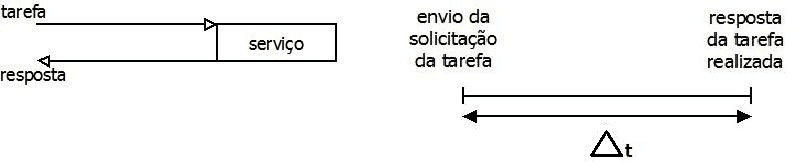
\includegraphics{../figuras/cap15-tempo-resposta.png}
\caption[Figura 15.1 -- Tempo de resposta de uma tarefa: o intervalo entre a solicitação e a resposta realizada]{Figura 15.1 -- Tempo de resposta de uma tarefa: o intervalo entre a solicitação e a resposta realizada. \textbf{Fonte:} \emph{Livro SCADA --- versão para análise}, p.~33 (Machado, Pontes e Vianna, reproduzida com crédito).}
\end{figure}

O tempo de resposta de um sistema SCADA é a \textbf{soma} dos tempos de cada subsistema envolvido ---
sensoriamento, ciclo do controlador, driver, rede, processamento na estação e desenho na tela. Como
as estações de supervisão não são determinísticas (\emph{Windows} ou \emph{Linux} com carga variável), o valor
exato não pode ser calculado a priori: ele é estimado, configurado e medido em campo.

O erro clássico de projeto é dimensionar a comunicação como se toda a banda configurada estivesse
disponível para dados. Em uma serial de 19.200 bps, cada \emph{frame} gasta bits de partida, de parada e
de verificação: sobra cerca de \textbf{dois terços} da banda para o dado útil. Em um intervalo de
atualização de 100 ms, isso significa algo em torno de 1.280 bits de dado --- suficiente para poucas
dezenas de variáveis, não para o cadastro inteiro.

\hypertarget{o-evento-que-se-perde-entre-as-varreduras}{%
\subsection{O evento que se perde entre as varreduras}\label{o-evento-que-se-perde-entre-as-varreduras}}

Há uma consequência mais grave que o atraso: o controlador pode \textbf{ver} um sinal que o supervisório
\textbf{não registra}. Se um pressostato atua por 20 ms e provoca o desligamento da planta, o CLP executa
o intertravamento no seu ciclo de varredura de poucos milissegundos --- mas a atualização da IHM pode
levar um segundo, e o alarme nunca aparece. A planta parou, e a tela não mostra por quê.

Esse é o tipo de falha mais difícil de investigar, porque não deixa rastro. A solução não é reduzir
a taxa do sistema inteiro --- é \textbf{capturar o evento no controlador}, onde a resolução é suficiente, e
transferir o resultado, e não o sinal.

\begin{caixafigura}

\textbf{{[}Figura 15.2 -- Configuração de tópicos com tempos de varredura distintos em um servidor de comunicação{]}}
\emph{Captura de tela de configuração de driver com três grupos de tags e a respectiva taxa: grupo rápido (200 ms) com variáveis de intertravamento e estado de bombas; grupo médio (1 s) com medições analógicas de processo; grupo lento (10 s) com totalizadores, temperaturas de mancal e diagnóstico. Ao lado, o campo de faixa morta por tag. Destacar que a classificação por dinâmica, não por área da planta, é o critério da divisão.}

\end{caixafigura}

\begin{center}\rule{0.5\linewidth}{0.5pt}\end{center}

\hypertarget{tratamento-o-que-se-faz-com-o-dado-antes-de-mostruxe1-lo}{%
\section{Tratamento: o que se faz com o dado antes de mostrá-lo}\label{tratamento-o-que-se-faz-com-o-dado-antes-de-mostruxe1-lo}}

Tratamento não é maquiagem: é a parte do projeto que separa informação de ruído. As operações usuais,
na ordem em que costumam ser aplicadas:

\begin{center}
\IfFileExists{../figuras/capitulo-15-m2.pdf}{%
  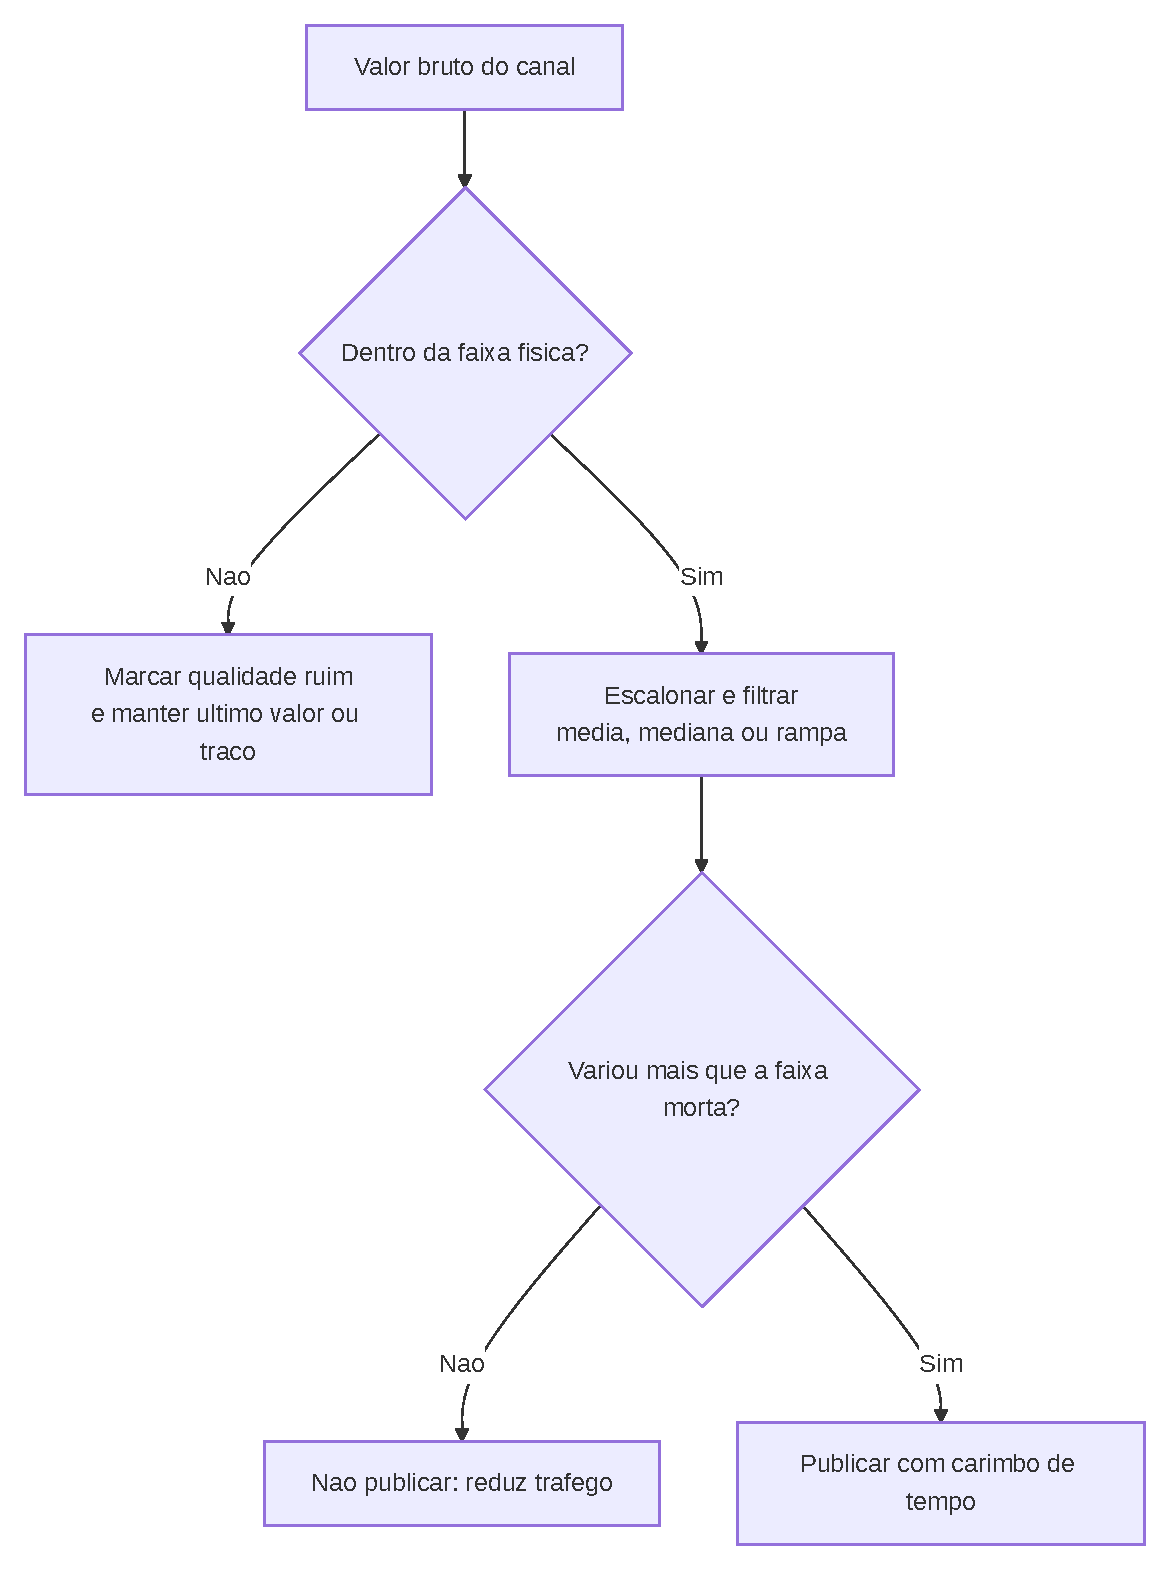
\includegraphics[width=\linewidth,height=0.8\textheight,keepaspectratio]{../figuras/capitulo-15-m2.pdf}%
}{\fbox{\parbox{0.9\linewidth}{\small Diagrama Mermaid ainda não renderizado: capitulo-15-m2. Rode scripts/render-mermaid.sh.}}}
\end{center}

\textbf{Tabela 15.4 -- Operações de tratamento e o risco de cada uma}

\begin{longtable}[]{@{}
  >{\raggedright\arraybackslash}p{(\columnwidth - 4\tabcolsep) * \real{0.3333}}
  >{\raggedright\arraybackslash}p{(\columnwidth - 4\tabcolsep) * \real{0.3333}}
  >{\raggedright\arraybackslash}p{(\columnwidth - 4\tabcolsep) * \real{0.3333}}@{}}
\toprule\noalign{}
\begin{minipage}[b]{\linewidth}\raggedright
Operação
\end{minipage} & \begin{minipage}[b]{\linewidth}\raggedright
Para que serve
\end{minipage} & \begin{minipage}[b]{\linewidth}\raggedright
Efeito colateral
\end{minipage} \\
\midrule\noalign{}
\endhead
\bottomrule\noalign{}
\endlastfoot
Validação de faixa & Rejeitar leituras fisicamente impossíveis (fora da faixa do sensor) & Faixa mal cadastrada rejeita dado bom \\
Escalonamento & Levar o valor bruto à unidade de engenharia & Divergência de faixa entre instrumento e cadastro gera erro silencioso \\
Média móvel & Reduzir ruído aleatório & Atrasa a resposta; mascara transitório real \\
Mediana móvel & Remover picos espúrios isolados & Custa mais processamento que a média \\
Faixa morta (\emph{deadband}) & Evitar publicação de variação irrelevante & Faixa morta alta esconde a tendência lenta \\
Publicação por exceção & Reduzir tráfego na rede e no enlace remoto & Exige \emph{refresh} periódico para não deixar a tela ``congelada'' \\
\end{longtable}

O critério para escolher entre eles não é estético. Em uma variável de proteção, o filtro deve ser o
menor possível ou inexistente; em uma variável de indicação lenta, como temperatura de mancal, um
filtro largo e uma faixa morta generosa reduzem tráfego sem prejuízo.

\begin{caixaatencao}

\textbf{Atenção:} filtro e faixa morta se somam. Um canal com média de 10 amostras e faixa morta de
2 \% pode levar mais de dois minutos para anunciar uma variação real de 1,5 \% --- e o operador só vai
descobrir isso no dia em que precisar da resposta rápida. Documente, para cada tag, o filtro e a
faixa morta configurados.

\end{caixaatencao}

\begin{center}\rule{0.5\linewidth}{0.5pt}\end{center}

\hypertarget{registro-da-primeira-falha}{%
\section{Registro da primeira falha}\label{registro-da-primeira-falha}}

Quando uma planta para, quase sempre vários instrumentos atuam em sequência: os intertravamentos
abraem, as bombas desligam, os pressostatos comutam. Se todos os eventos chegam ao supervisório com
carimbo de tempo do próprio supervisório, a ordem aparente é apenas a ordem de chegada --- e a causa
raiz se perde na avalanche.

O \textbf{registrador de primeiro evento} resolve isso dentro do controlador: cada linha de
intertravamento ganha, logo abaixo, um bloco que grava o código do sensor em um endereço de memória
e aciona um bit de bloqueio. Do segundo sensor em diante, o bloqueio impede a sobrescrita. O
supervisório lê apenas um endereço --- o código do primeiro sensor que atuou.

\begin{figure}
\centering
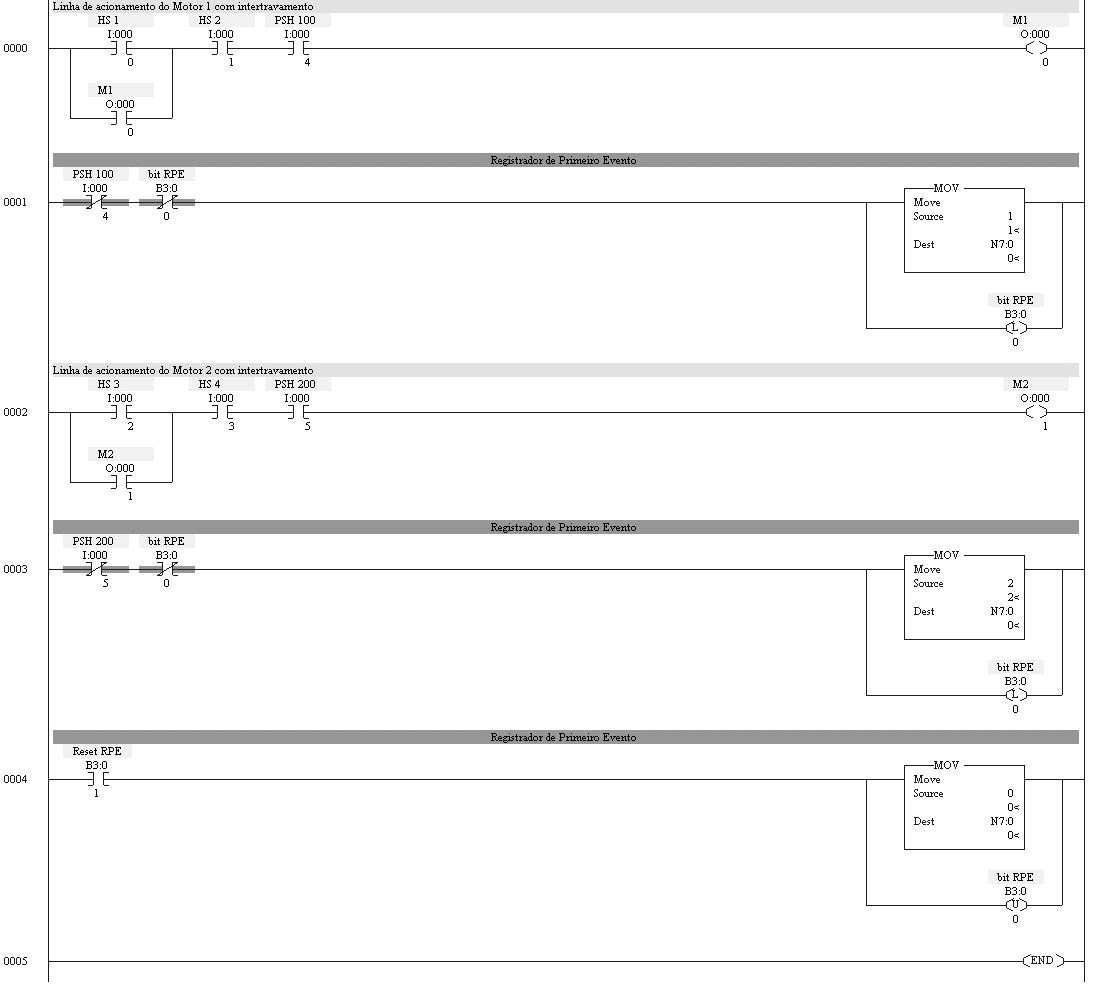
\includegraphics{../figuras/cap15-registrador-primeiro-evento.png}
\caption[Figura 15.3 -- Lógica em Ladder do registrador de primeiro evento, com bit de bloqueio e blocos Move]{Figura 15.3 -- Lógica em Ladder do registrador de primeiro evento, com bit de bloqueio e blocos Move. \textbf{Fonte:} \emph{Livro SCADA --- versão para análise}, p.~36 (Machado, Pontes e Vianna, reproduzida com crédito).}
\end{figure}

\textbf{Tabela 15.5 -- Tabela de alocação do registrador de primeiro evento}

\begin{longtable}[]{@{}
  >{\raggedright\arraybackslash}p{(\columnwidth - 4\tabcolsep) * \real{0.3333}}
  >{\raggedright\arraybackslash}p{(\columnwidth - 4\tabcolsep) * \real{0.3333}}
  >{\raggedright\arraybackslash}p{(\columnwidth - 4\tabcolsep) * \real{0.3333}}@{}}
\toprule\noalign{}
\begin{minipage}[b]{\linewidth}\raggedright
Endereço
\end{minipage} & \begin{minipage}[b]{\linewidth}\raggedright
Tagname
\end{minipage} & \begin{minipage}[b]{\linewidth}\raggedright
Descrição
\end{minipage} \\
\midrule\noalign{}
\endhead
\bottomrule\noalign{}
\endlastfoot
\passthrough{\lstinline!I:000/0!} & \passthrough{\lstinline!HS 1!} & Chave de acionamento do motor 1 (NA) \\
\passthrough{\lstinline!I:000/1!} & \passthrough{\lstinline!HS 2!} & Chave de desacionamento do motor 1 (NF) \\
\passthrough{\lstinline!I:000/4!} & \passthrough{\lstinline!PSH 100!} & Chave de pressão alta (NF) \\
\passthrough{\lstinline!I:000/5!} & \passthrough{\lstinline!PSH 200!} & Chave de pressão alta (NF) \\
\passthrough{\lstinline!B3:0/0!} & \passthrough{\lstinline!bit RPE!} & Bit de bloqueio que impede alteração do valor gravado \\
\passthrough{\lstinline!B3:0/1!} & \passthrough{\lstinline!Reset RPE!} & Botão que reinicia o registrador pela IHM \\
\passthrough{\lstinline!N7:0!} & \passthrough{\lstinline!Codigo RPE!} & Número do sensor que originou a parada \\
\end{longtable}

Três cuidados determinam se a lógica funciona na prática:

\begin{enumerate}
\def\labelenumi{\arabic{enumi}.}
\tightlist
\item
  \textbf{A linha de registro fica imediatamente abaixo do intertravamento correspondente.} Se ela for
  deslocada, o tempo de varredura pode fazer o código do segundo sensor chegar antes do primeiro.
\item
  \textbf{Existe uma lista de relação entre número e evento}, homologada e disponível para a operação ---
  sem ela, o código gravado na memória é um número sem significado.
\item
  \textbf{O registrador é reiniciado pela IHM}, com registro de quem reiniciou e quando.
\end{enumerate}

\begin{caixanota}

\textbf{Atualização tecnológica:} o registrador em Ladder continua válido e é a solução mais barata
em controladores que não têm cartão de sequência de eventos. Em arquiteturas atuais, a mesma
função é obtida com \textbf{RTUs e controladores com SOE} (\emph{Sequence of Events}), que carimbam cada
entrada com resolução de milissegundo na origem, e com \textbf{sincronização de tempo} por NTP ou
PTP (IEEE 1588) em toda a planta. A escolha depende do que se quer provar: a lógica em Ladder diz
\emph{qual} foi o primeiro a atuar; o SOE com carimbo na origem diz \emph{quando}, com resolução suficiente
para reconstruir a sequência inteira.

\end{caixanota}

O carimbo de tempo é o outro lado do problema. Dados carimbados na chegada ao supervisório perdem a
ordem real, sobretudo em enlaces com atraso variável. A regra é simples: \textbf{carimbe na origem}
sempre que o equipamento permitir, e mantenha os relógios de todos os nós sincronizados --- um
histórico com relógios discrepantes é pior que um histórico sem relógio, porque produz conclusões
erradas com aparência de precisão.

\begin{center}\rule{0.5\linewidth}{0.5pt}\end{center}

\hypertarget{comparativo-das-arquiteturas-de-aquisiuxe7uxe3o}{%
\section{Comparativo das arquiteturas de aquisição}\label{comparativo-das-arquiteturas-de-aquisiuxe7uxe3o}}

Quatro arranjos resolvem a aquisição, e a escolha depende do que existe no campo e do que se
pretende fazer com o dado.

\textbf{Tabela 15.6 -- Comparativo das arquiteturas de aquisição}

\begin{longtable}[]{@{}
  >{\raggedright\arraybackslash}p{(\columnwidth - 10\tabcolsep) * \real{0.1667}}
  >{\raggedright\arraybackslash}p{(\columnwidth - 10\tabcolsep) * \real{0.1667}}
  >{\raggedright\arraybackslash}p{(\columnwidth - 10\tabcolsep) * \real{0.1667}}
  >{\raggedright\arraybackslash}p{(\columnwidth - 10\tabcolsep) * \real{0.1667}}
  >{\raggedright\arraybackslash}p{(\columnwidth - 10\tabcolsep) * \real{0.1667}}
  >{\raggedright\arraybackslash}p{(\columnwidth - 10\tabcolsep) * \real{0.1667}}@{}}
\toprule\noalign{}
\begin{minipage}[b]{\linewidth}\raggedright
Tecnologia
\end{minipage} & \begin{minipage}[b]{\linewidth}\raggedright
Função
\end{minipage} & \begin{minipage}[b]{\linewidth}\raggedright
Protocolo
\end{minipage} & \begin{minipage}[b]{\linewidth}\raggedright
Aplicação
\end{minipage} & \begin{minipage}[b]{\linewidth}\raggedright
Vantagens
\end{minipage} & \begin{minipage}[b]{\linewidth}\raggedright
Limitações
\end{minipage} \\
\midrule\noalign{}
\endhead
\bottomrule\noalign{}
\endlastfoot
CLP com cartões de I/O & Aquisição e controle no mesmo equipamento & Modbus, OPC UA, PROFINET, EtherNet/IP & Processo com lógica de controle local & Lógica e aquisição juntas; varredura rápida; diagnóstico de canal & Custo por ponto maior em instalações muito distribuídas \\
Sistema DAQ & Aquisição dedicada, sem controle & Modbus, OPC, proprietário & Bancada, ensaio, monitoramento de máquina & Alta resolução e taxa; pronto para ensaio & Sem controle, sem intertravamento \\
RTU & Aquisição remota com transmissão & DNP3, IEC 60870-5-101/104, Modbus & Campo remoto, baixo consumo & Baixo consumo, robustez, comunicação por rádio ou celular & Menor capacidade de lógica; programação menos padronizada \\
Gateway de borda & Aquisição, normalização e publicação & Modbus, OPC UA, MQTT, REST & Integração com nuvem e múltiplos protocolos & Concentra protocolos, faz \emph{store and forward}, reduz tráfego & É mais um nó para manter, atualizar e proteger \\
\end{longtable}

A tendência de projeto não é escolher um deles para toda a planta, e sim \textbf{usar cada um onde ele é
melhor}: CLP onde há controle e intertravamento, RTU onde há campo remoto, gateway onde há
integração. O Capítulo 18 trata da integração entre eles.

\begin{center}\rule{0.5\linewidth}{0.5pt}\end{center}

\hypertarget{estudo-de-caso-a-planta-que-parou-e-a-tela-nuxe3o-mostrou-por-quuxea}{%
\section{\texorpdfstring{Estudo de Caso --- A planta que parou e a tela não mostrou por quê}{Estudo de Caso  A planta que parou e a tela não mostrou por quê}}\label{estudo-de-caso-a-planta-que-parou-e-a-tela-nuxe3o-mostrou-por-quuxea}}

\textbf{Cenário.} Uma planta de tratamento de água com duas bombas de recalque e duas chaves de pressão
alta. Em três semanas, o conjunto parou quatro vezes por atuação da proteção. Em todas as
ocorrências, o histórico de alarmes registrou, com diferença de poucos segundos, o alarme de ``pressão
alta'' e o de ``bomba desligada'' --- sem indicação confiável de qual veio primeiro. A manutenção
trocou um pressostato, verificou o outro e não encontrou defeito.

\textbf{Diagnóstico.} Três problemas somados:

\begin{enumerate}
\def\labelenumi{\arabic{enumi}.}
\tightlist
\item
  O carimbo de tempo de todos os alarmes era atribuído pelo supervisório, na chegada --- não na
  origem.
\item
  A varredura do driver para as chaves de pressão era de 1 s, maior que a duração do pulso de
  pressão alta no instante da atuação.
\item
  Os dois pressostatos atuavam em sequência por projeto (um é proteção, o outro é alarme), o que
  torna indistinguível a ``primeira'' atuação se os dois eventos chegam com o mesmo carimbo.
\end{enumerate}

\textbf{Decisão de engenharia.}

\begin{longtable}[]{@{}
  >{\raggedright\arraybackslash}p{(\columnwidth - 2\tabcolsep) * \real{0.5000}}
  >{\raggedright\arraybackslash}p{(\columnwidth - 2\tabcolsep) * \real{0.5000}}@{}}
\toprule\noalign{}
\begin{minipage}[b]{\linewidth}\raggedright
Medida
\end{minipage} & \begin{minipage}[b]{\linewidth}\raggedright
Efeito
\end{minipage} \\
\midrule\noalign{}
\endhead
\bottomrule\noalign{}
\endlastfoot
Registrador de primeiro evento no CLP, com código por sensor e lista homologada & Passa a existir um único registro confiável de primeira atuação \\
Chaves migradas para o grupo de varredura rápido (200 ms) do driver & A atuação passa a ser observada, e não apenas inferida \\
Sincronização dos relógios do CLP, da estação e do servidor & Os carimbos de tempo passam a ser comparáveis \\
Alarme de ``primeira atuação da proteção'' distinto do alarme de processo & A operação deixa de receber dois alarmes concorrentes sem hierarquia \\
\end{longtable}

\textbf{Resultado.} Na ocorrência seguinte, o registro apontou \passthrough{\lstinline!PSH 100!} como primeira atuação, nove
segundos antes do desligamento --- a causa era uma válvula de retenção que fechava lentamente e
provocava golpe de aríete. O defeito era de processo, não do instrumento, e nenhuma das quatro
ocorrências anteriores permitiria essa conclusão.

\textbf{Limitações do arranjo.} O registrador de primeiro evento informa \emph{qual} foi o primeiro, não
\emph{quando} com precisão de milissegundo. Para análise de sequência real, a solução é cartão de SOE com
carimbo na origem e PTP. Além disso, a lógica em Ladder precisa ser revista sempre que um novo
intertravamento é acrescentado --- e essa manutenção precisa estar no procedimento de gestão de
mudanças, não na memória de quem programou.

\begin{center}\rule{0.5\linewidth}{0.5pt}\end{center}

\hypertarget{resumo}{%
\section{Resumo}\label{resumo}}

\begin{itemize}
\tightlist
\item
  A aquisição é uma \textbf{cadeia de elos}, e cada um acrescenta erro, atraso ou descarte.
\item
  O \textbf{4 mA} da faixa de 4 a 20 mA existe para separar ``valor zero'' de ``sem sinal''.
\item
  \textbf{Resolução, exatidão e ruído} são grandezas distintas; a resolução do conversor raramente é o gargalo.
\item
  Cada elo tem o seu ritmo: o ciclo do controlador é de milissegundos, a atualização da IHM é de décimos de segundo a segundos.
\item
  O tempo de resposta é a \textbf{soma} dos subsistemas e não é determinístico nas estações de supervisão.
\item
  Eventos curtos podem atuar no intertravamento e \textbf{não aparecer} no supervisório --- a solução é capturar no controlador.
\item
  \textbf{Tratamento} (validação, escalonamento, filtração e faixa morta) separa informação de ruído, mas cada operação tem custo: atraso e perda de transitório.
\item
  A \textbf{primeira falha} de uma parada precisa ser registrada na origem; lógica em Ladder resolve o ``qual'', o SOE com carimbo resolve o ``quando''.
\item
  Relógios sincronizados são pré-requisito para qualquer análise de sequência.
\end{itemize}

\hypertarget{questuxf5es-de-revisuxe3o}{%
\section{Questões de Revisão}\label{questuxf5es-de-revisuxe3o}}

\begin{enumerate}
\def\labelenumi{\arabic{enumi}.}
\tightlist
\item
  Descreva a cadeia de aquisição de uma medição de nível, citando o que cada elo pode fazer com o dado.
\item
  Por que a faixa de 4 a 20 mA começa em 4 mA e qual a consequência prática de ler zero nessa entrada?
\item
  Explique a diferença entre resolução, exatidão e ruído, usando o exemplo de um transmissor de 0,5 \% ligado a um cartão de 16 bits.
\item
  Um sistema tem ciclo de varredura de 10 ms no CLP, varredura de driver de 1 s e atualização de IHM de 2 s. Um sinal permanece alto por 300 ms. Descreva o que cada elo registra e qual o risco para a operação.
\item
  Por que o tempo de resposta de um sistema SCADA não pode ser calculado com precisão antes da instalação? Cite três fatores que o influenciam.
\item
  Explique como funciona o registrador de primeiro evento e por que a linha de registro precisa ficar logo abaixo do intertravamento correspondente.
\item
  Compare filtro de média e faixa morta quanto ao efeito sobre ruído, atraso e volume de tráfego.
\item
  Um histórico de alarmes mostra dois eventos com o mesmo carimbo de tempo. Que deficiências de projeto podem explicar isso e como corrigi-las?
\item
  Compare CLP, sistema DAQ, RTU e gateway de borda quanto à função, protocolo e limitação principal, e indique um cenário em que os quatro convivem na mesma planta.
\end{enumerate}

\hypertarget{referuxeancias}{%
\section{Referências}\label{referuxeancias}}

\begin{itemize}
\tightlist
\item
  MACHADO, R.; PONTES, W.; VIANNA, W. \textbf{Livro SCADA --- versão para análise}. Material didático do curso (seções sobre desempenho do sistema de automação SCADA, sistemas de tempo real e registrador de primeiro evento). Figuras reproduzidas com crédito.
\item
  VIANNA, W. S. \textbf{Sistema SCADA Supervisório}. IFF, 2008 (capítulos sobre componentes de hardware e software, drivers de comunicação e elementos dinâmicos).
\item
  FARINES, J. M.; FRAGA, J. S.; OLIVEIRA, R. S. \textbf{Sistemas de Tempo Real}. São Paulo: Escola de Computação, 2000 (definição de sistema de tempo real citada na obra de origem).
\item
  INTERNATIONAL ELECTROTECHNICAL COMMISSION. \textbf{IEC 61131-3 --- Programmable controllers: Programming languages}. 4ª edição, maio de 2025.
\item
  INSTITUTE OF ELECTRICAL AND ELECTRONICS ENGINEERS. \textbf{IEEE 1588 --- Precision Clock Synchronization Protocol for Networked Measurement and Control Systems} (PTP; verificar edição vigente).
\item
  INTERNATIONAL SOCIETY OF AUTOMATION. \textbf{ANSI/ISA-5.1 --- Instrumentation Symbols and Identification} (identificação de instrumentos por letras; verificar edição vigente antes de citar em projeto).
\item
  ISA. \textbf{ISA-101 --- Human-Machine Interfaces for Process Automation Systems} (referência geral de apresentação de dados ao operador; verificar edição vigente).
\item
  OPC FOUNDATION. \textbf{OPC Unified Architecture} --- \emph{subscription}, intervalo de amostragem e \emph{deadband} por item monitorado. Disponível em: opcfoundation.org. Consulta: 2026.
\end{itemize}
